\documentclass[sigconf]{acmart}
%% \documentclass[manuscript,screen]{acmart}
\usepackage{titlesec}

\titleformat*{\subsubsection}{\large \bfseries}

%% \BibTeX command to typeset BibTeX logo in the docs
\AtBeginDocument{%
  \providecommand\BibTeX{{%
    \normalfont B\kern-0.5em{\scshape i\kern-0.25em b}\kern-0.8em\TeX}}}

%%\acmSubmissionID{123-A56-BU3}

%%\citestyle{acmauthoryear}

%%
%% end of the preamble, start of the body of the document source.
\begin{document}

\title{Milestone 2 -- Supervised Learning}

\author{Maciej Nalepa}
\affiliation{}
\email{maciej.nalepa@alu.uclm.es}

\author{Piotr Maliszewski}
\affiliation{}
\email{piotr.maliszewski@alu.uclm.es}

\author{Gökay Iseri}
\affiliation{}
\email{gokay.iseri@alu.uclm.es}

\author{Başar Milli}
\affiliation{}
\email{basar.milli@alu.uclm.es}

\renewcommand{\shortauthors}{Nalepa Maliszewski Iseri Milli}

\begin{abstract}
The purpose of this work is to train a regressor model on the environmental data collected by various U.S.
Federal Government Agencies from two cities ( San Juan, Puerto Rico and Iquitos, Peru) to
gain a better understanding of the Denge Spread Phenomena.
These data are from a competition of the site DrivenData. 
The overall objective is to use supervised learning techniques to predict the number of cases on the basis of the collected data and create a model that will successfully predict them.
Training data will be used to acquire a model and test data will be used to generate submissions and evaluate score among other competitors.

\end{abstract}

%%
%% http://dl.acm.org/ccs.cfm
%%
\begin{CCSXML}
<ccs2012>
   <concept>
       <concept_id>10010147.10010257</concept_id>
       <concept_desc>Computing methodologies~Machine learning</concept_desc>
       <concept_significance>500</concept_significance>
       </concept>
 </ccs2012>
\end{CCSXML}

\ccsdesc[500]{Computing methodologies~Machine learning}

\keywords{machine learning, supervised}

\maketitle

%
%   +++++++OUR CODE
%

\section{Introduction}
In this project we explore supervised Learning methods.
We were working on DrivenData DengAI: Predicting Disease Spread competition dataset.
The whole dataset was used to achieve possibly best prediction results.
However, there is an option to limit the data to the subset that was initially assigned to our working group.

\subsection{Project files}
The code and source files are available at  \url{https://github.com/GummyBearStudioTeam/ESI_MLTechniques}.

\section{Data Preprocessing}
The data was preprocessed by filling NaN values using backward fill method, later scaled with a standard scaler. For experimenting PCA was applied to generate alternative version of the dataset.

\begin{table}[h]
    \begin{tabular}{|l|r|r|}
    \hline
    city & mean  & var  \\ \hline
    sj   & 34.18 & 2640 \\
    iq   & 7.57  & 116  \\ \hline
    \end{tabular}
    \centering
    \caption{Labels mean and variance values.}
\end{table}

Distribution of the labels which is the $total\_cases$ value is highly unbalanced (\ref{totalcases}). Its mean is much lower than the variance.
To potentially improve performance of linear models a logarithmic transformation has been applied to these labels in order to acquire a distribution closer to a standard distribution (\ref{totalcasesnormal}).

\begin{figure}[h]
    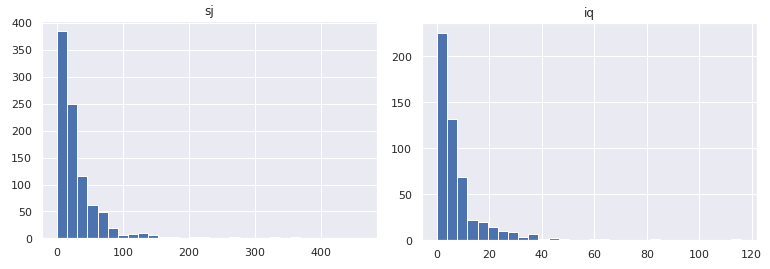
\includegraphics[width=\linewidth]{total-cases.png}
    \centering
    \caption{Distribution of the $total\_cases$ before transformation.}
    %\Description{}
    \label{totalcases}
\end{figure}
\begin{figure}[h]
    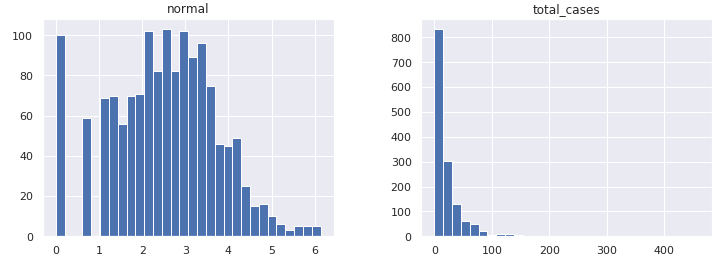
\includegraphics[width=\linewidth]{normal-total-cases.png}
    \centering
    \caption{Distribution of the $total\_cases$ with logarithmic transformation (left-hand side).}
    %\Description{}
    \label{totalcasesnormal}
\end{figure}

Basic analysis steps have been performed to select best features and clean the dataset from highly correlated variables. Variables with absolute correlation higher than $0.8$ were paired and marked for removal. The removed variable from each pair was chosen by its importance which is the correlation value with the label (\ref{importance}).

\begin{figure}[h]
    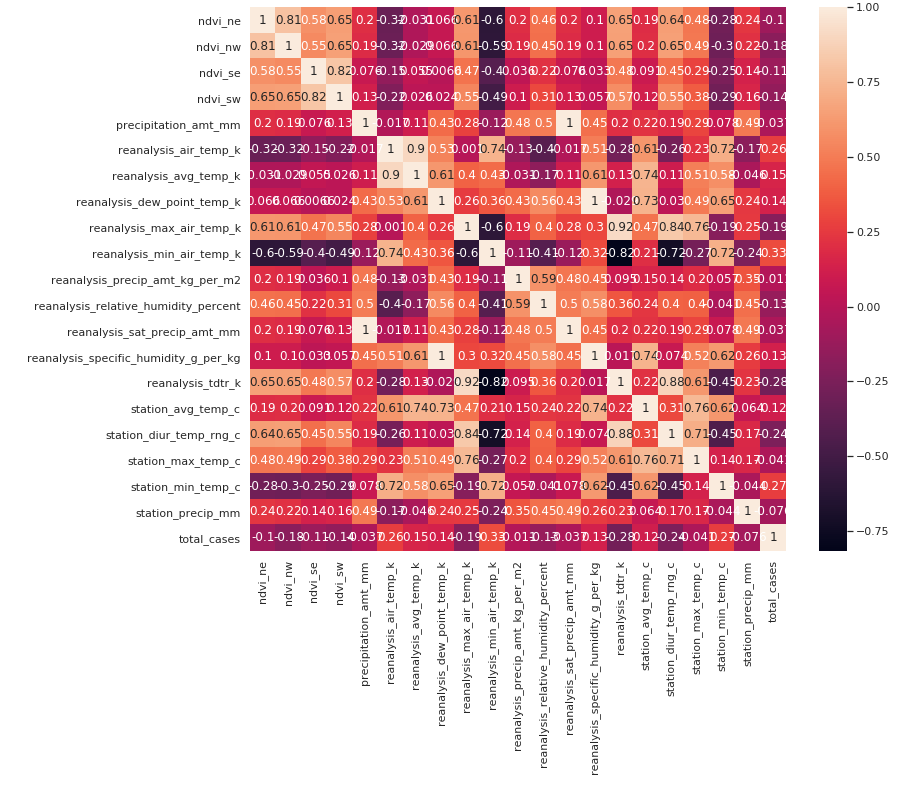
\includegraphics[width=\linewidth]{corr.png}
    \centering
    \caption{Data correlation matrix. Note that some variables have correlation reaching $1$.}
    %\Description{}
    \label{corr}
\end{figure}
\begin{figure}[h]
    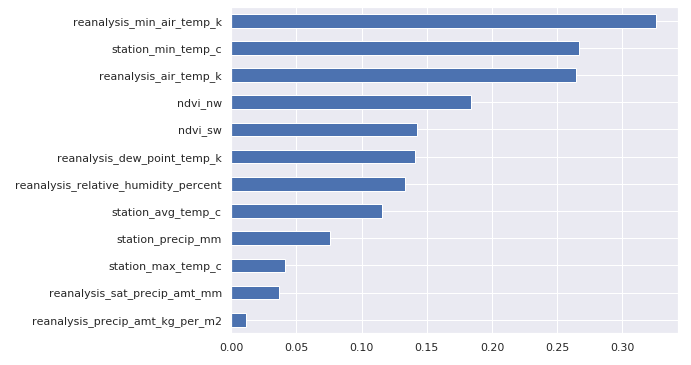
\includegraphics[width=\linewidth]{importance.png}
    \centering
    \caption{Cleaned features importance values.}
    %\Description{}
    \label{importance}
\end{figure}

Importance analysis was performed also on the PCA transformed dataset.
The mean importance of the cleaned features was $0.145$, while the PCA features scored around $0.062$.
This can result in the models trained with PCA as input to perform worse than default ones.

\section{Models}
The goal is to find most robust regression model that will successfully predict the values on the unlabeled test data.
We propose an approach of training 2 separate models for the city of San Juan and Iquitos as they show much different characteristics.
What is more, we split the data for training and testing with the ratio of $15\%$ for testing. Which is supposed to help determine a better model for prediction against the target unlabeled data.

Each training can be easily configured to run on different data in the notebook.
Possible changes are the city, transformed or non-transformed labels and PCA transformed features.
There is also an option to drop a set amount of least important features.

Following regression models have been selected to predict the values of our data:
\begin{itemize}
    \item k-Nearest Neighbors -- which serves as a baseline model
    \item Decision Tree
    \item Random Forest
    \item Linear Support Vector
\end{itemize}

We are also using the boosting models which are:
\begin{itemize}
    \item Ada Boost
    \item Gradient Boosting
\end{itemize}

The metric score used was Mean Absolute Error.
For obtaining a quality score of each model a fold on the training set was applied and maximum MAE was returned as the score of the model.

\subsection{kNN}
KNN regressor can use different weights during training.
We tested its performance with default weight functions \emph{uniform} and \emph{distance} settings.
For each branching system was tested checking consecutively next values of \emph{n\_neighbour} which is the number of  neighbours to use in KNN algorithm.
Performance of this model was our baseline which we try to improve.

\begin{figure}[h]
    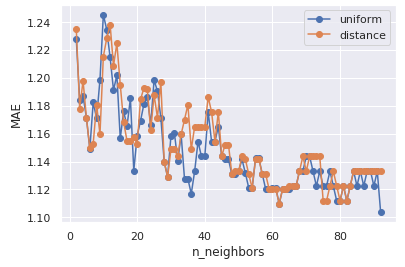
\includegraphics[width=\linewidth]{1-knn.png}
    \centering
    \caption{MAE of kNN. (low MAE values are the result of using transformed labels)}
    %\Description{}
\end{figure}

\subsection{Decision Tree}
The most important parameter for a Decision Tree regressor is the maximal depth of the tree.
We tested its performance in the range between 2 and 40.
Greater numbers haven't been decreasing the error.

This model can be an improvement over kNN.

\begin{figure}[h]
    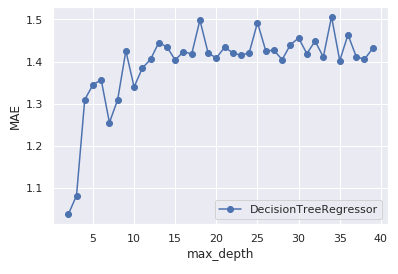
\includegraphics[width=\linewidth]{2-decision-tree.png}
    \centering
    \caption{MAE of Decision Tree.}
    %\Description{}
\end{figure}

\subsection{Random Forest}
We have been checking various values of \emph{max\_estimators} parameter and various \emph{max\_depths}. 
Values of max\_estimators have been checked in the range from 2 to 7, while max\_depth varied from 2 up to 20.

This model can be an improvement over kNN.

\begin{figure}[h]
    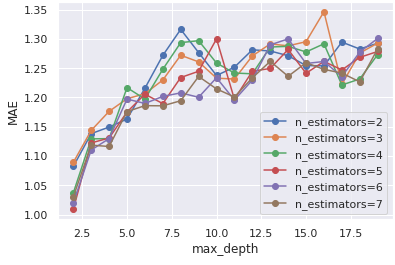
\includegraphics[width=\linewidth]{3-random-forest.png}
    \centering
    \caption{MAE of Random Forest.}
    %\Description{}
\end{figure}

\subsection{Linear SVR}
Another tested regressor is Linear SVR which was optimized by tuning its regularization parameter $C$. The value was analyzed in the logarithmic space in the range between $10^{-5} ; 10^{0.5}$.

Generally this model turned out to be one of the least effective.

\begin{figure}[h]
    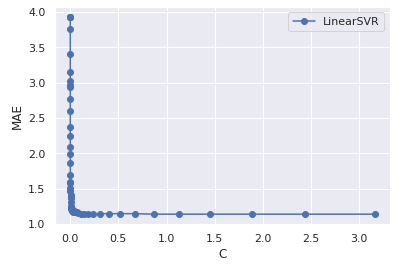
\includegraphics[width=\linewidth]{4-linear-svr.png}
    \centering
    \caption{MAE of Linear SVR.}
    %\Description{}
\end{figure}

\subsection{Visualisation}
Each model has its visualisation, which is a plot showing the predicted and actual values.

\begin{figure}[h]
    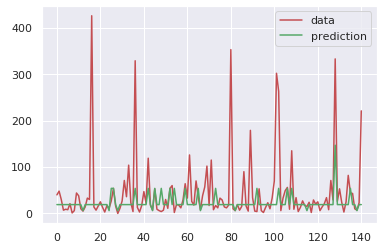
\includegraphics[width=\linewidth]{5-eval.png}
    \centering
    \caption{Example prediction visualisation on a test set.}
    %\Description{}
\end{figure}

\section{Optimization}
\subsection{Boosting}
Ada Boost with decision tree of depth $3$ and Gradient Boosting are the two boosting regressors chosen for further experimenting.
Feature importance were measured on these two models and compared with default Decision Tree and Random Forest.

Models with boosting have the distribution of importance more evenly distributed in comparison to the other two.

\begin{figure}[h]
    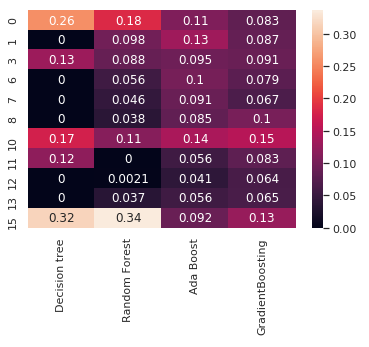
\includegraphics[width=\linewidth]{6-feature-boosting.png}
    \centering
    \caption{Boosting: feature importance (PCA features).}
    %\Description{}
\end{figure}

\subsection{Parameter Search}
We have performed a Grid Search and Random Search to optimize Random Forest Regressor model.
The best discovered models were added to the collection of all models fitted to the data for further analysis.

For the model collection we calculate MAE on the whole dataset, MAE on test dataset, R2 score on the whole dataset and a product of the first two absolute errors called MAE2.

\begin{figure}[h]
    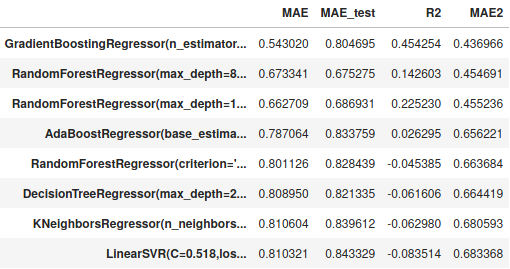
\includegraphics[width=\linewidth]{7-model-eval.png}
    \centering
    \caption{Model evaluation and selection for submission.}
    %\Description{}
\end{figure}

\subsection{Submission}
In total 11 submissions were performed. Some turned out to be erroneous and had to be repeated.
The submission files are available in the \texttt{submission} directory and they have their corresponding metrics file in the \texttt{metrics} directory.

Best score submission does not have a corresponding metric because it was generated during testing in the work in progress phase of our project. The result could not be improved with presented approach.

A screenshot confirming obtained results is available as \texttt{submission/screenshot.png}.

\begin{table}[h]
    \begin{tabular}{|l|l|}
    \hline
    submission   & score   \\ \hline
    best         & 28.9808 \\
    PCA + normal & 29.1370 \\
    default      & 29.3486 \\
    normal       & 29.4904 \\ \hline
    \end{tabular}
    \caption{Submission scores.}
\end{table}

\begin{figure}[h]
    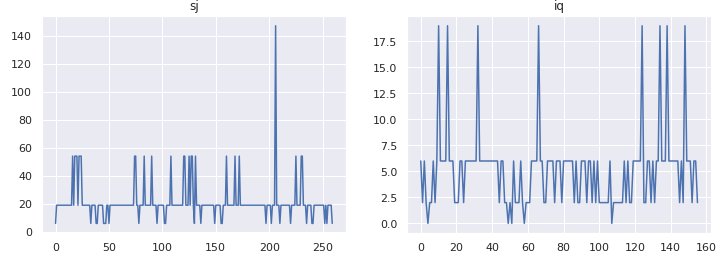
\includegraphics[width=\linewidth]{8-prediction.png}
    \centering
    \caption{Example of final submission predictions for the cities of San Juan and Iquitos.}
    %\Description{}
\end{figure}

\section{Refinement}
The project could extend the optimization part, possibly a deeper analysis of some parameters in the presented models can be achieved. For example, Gradient Boosting was using a constant value of \emph{n estimators}.

Also some others regression models could be implemented that can be an improvement over the currently best scoring solutions.

The problem could be treated as a time-series forecasting problem, a recurrent model may perform better on this dataset.

\section{Summary}
We have presented our approach to the supervised learning regression problem of the disease spread prediction.

Multiple regression models were tested and optimized for acquiring the most accurate parameters possible in reasonable time.
Manual optimization, boosting and automatic search were used to generate a collection of models from which the best was picked.

Although the presented models have failed to best the drivendata benchmark model, they have bested the performance of our baseline kNN model, which was usually scoring at the bottom end results in our metrics.

%
%   -------OUR CODE
%

%% The acknowledgments section is defined using the "acks" environment
%% (and NOT an unnumbered section). This ensures the proper
%% identification of the section in the article metadata, and the
%% consistent spelling of the heading.
\begin{acks}
This work is part of UCLM project of the Machine Learning Techniques subject. Group PMG.
\end{acks}

%%
%% The next two lines define the bibliography style to be used, and
%% the bibliography file.
%\bibliographystyle{ACM-Reference-Format}
%\bibliography{sample-base}

\end{document}
\endinput
%%
%% End of file `sample-xelatex.tex'.
